\chapter{Grundlagen}\label{chapter:Grundlagen}
Dieses Kapitel behandelt die Grundlagen, die für die Realisierung des Prototyps notwendig sind. Dabei werden Methoden und Eigenschaften der Augmented Reality erläutert, sowie ein Überblick über OpenGL gegeben.

\section{Augmented Reality}\label{AR}
In der Literatur lassen sich für den Begriff der Augmented Reality (AR, deutsch: \glqq angereicherte Realität\grqq ) viele unterschiedliche Definitionen finden, die meisten stützen sich dabei auf das von \citet{milgram:augmented-reality} definierte Reality-Virtuality (RV) Kontinuum, welches in Abbildung \ref{fig:RV-Kontinnum} dargestellt ist.\\
Um dieses zu verstehen muss zunächst der Bergriff der Virtual Reality (VR, deutsch: \glqq virtuelle Realität\grqq ) definiert werden. Nach \citet[S.1]{klein:visual-tracking} beschreibt die VR eine völlig künstliche, computergenerierte Welt, in die der Nutzer eintauchen kann. \\
Milgrams Definition fasst nun die Virtual Reality und die reale Welt als zwei, sich gegenüberliegende Enden eines Kontinuums auf. Dabei ist die reale Welt an die physikalischen Gesetze gebunden, während die virtuelle Welt diese überschreiten und sich von ihnen lösen kann \citep[S. 283]{milgram:augmented-reality}. Nach dem RV Kontinuum bewegt sich die Augmented Reality zwischen beiden Welten und stellt ein Kombination beider dar.
\begin{figure}[h!]
\centering
\includegraphics[width=0.8\textwidth]{Abbildungen/milgram-rv-continuum.jpeg}
\caption[RV Kontinuum]{Das Reality-Virtuality (RV) Kontinuum. (Quelle: \citet[S. 283]{milgram:augmented-reality})}
\label{fig:RV-Kontinnum}
\end{figure}
Eine weitere Definition, die sich auch mit der von Milgram vereinbaren lässt, beschreibt die Augmented Reality als eine computergestützte Erweiterung der wahrnehmbaren Realität um virtuelle Objekte \citep[S. 9]{tab:augmented-reality}. 
Auf dieser Grundlage kann man Augmented Reality als das Einbinden und Visualisieren digitaler, computergenerierte Objekte in der realen Welt auffassen.\\
Oftmals wird dabei das Ziel verfolgt eine möglichst realistische Illusion für den Nutzer zu schaffen.\\

\subsection{Einsatzbereiche}
Die erste Assoziation, die die meisten mit dem Begriff Augmented Reality verbinden ist vermutlich der Unterhaltungsbereich. Große Firmen wie zum Beispiel Snapchat nutzen die Technologie um kleine Gimmicks für ihre Nutzer bereitzustellen (siehe Abbildung \ref{fig:snapchat-ar})
Die meisten Personen, die den Begriff Augmented Reality hören, werden vermutlich an ein lustiges Gimmick zur Unterhaltung denken. Doch auch neben dem Bereich der Unterhaltung wird AR an vielen weiteren Stellen eingesetzt.\\
Beispielhaft zu nennen wären hier der Bereich der Produktion, in welchem AR unter Anderem als Hilfsmittel zum Prototyping \citep[S. 44]{tab:augmented-reality} genutzt werden kann, oder der Bereich der Medizin. Im letzteren können mittels AR Therapiemaßnahmen für psychische Erkrankungen oder Assistenzsysteme zur Diagnose und Operation entwickelt werden \citep[S. 52, 54]{tab:augmented-reality}.\\
Der Einsatzbereich in dessen Rahmen sich diese Arbeit bewegt ist jedoch der Bereich der Bildung.\\
Hier bietet Augmented Reality die Möglichkeit eines neuen Informationsmediums, welches vor allem zur Betrachtung dreidimensionaler Objekte genutzt werden kann. Dieses ermöglicht ein verbessertes, räumliches Verständnis des Lerninhaltes. 
Laut einer systematischen Analyse der Universität Stockholm, in welchem basierend auf der Anzahl der wissenschaftlichen Veröffentlichungen Schlüsse für das Lernen mit AR gezogen wurden, sind vor allem die Naturwissenschaften relevant für den Einsatz von AR  \citep[S. 81]{hedberg:review-ar-learning}. 

\begin{figure}[h!]
\centering
\includegraphics[width=0.5\textwidth]{Abbildungen/snapchat-ar.jpg}
\caption[Snapchat AR]{AR Gimmick aus der Anwendung Snapchat. (Quelle: Screenshot aus der Anwendung Snapchat, 01.08.2020)}
\label{fig:snapchat-ar}
\end{figure}

\subsection{Technische Grundlagen}
Zur Umsetzung der Augmented Reality ist eine Umgebungserfassung und -analyse des Systems mit Hilfe einer Tracking Software (auch Tracker genannt) notwendig. Auf Grundlage dieser können dann im Anschluss computergenerierte virtuelle Objekte in die Umgebung eingefügt werden. \\
Zur Analyse der Systemumgebung können verschiedene Eingabesysteme genutzt werden, mit deren Hilfe die Eigenschaften der Umgebung und der in ihr vorhandenen Objekte wahrgenommen werden können \citep[S. 22]{tab:augmented-reality}. Zu diesen Eigenschaften zählen neben statischen, wie der Größen und Position, auch dynamische Eigenschaften, welche die Veränderung der statischen Attribute einzelner Objekte umfassen \todo{Umformulieren, wegen Zitat}. Beispielhafte Technologien, die zur Erfassung genutzt werden können, wären Kamerasysteme, Laser, Infrarot oder sonstige Sensoren \citep[S. 22]{tab:augmented-reality}.
Neben der Umgebungserfassung ist auch die Verfolgung einzelner, in der Umgebung enthaltender Objekte notwendiger Bestandteil der Tracking Software, um die dynamischen Eigenschaften der realen Umgebung auf die virtuellen Objekte zu übertragen.\\
Eine wichtige Rolle beim Tracking spielt die Genauigkeit, mit der die Eigenschaften der Umgebung wahrgenommen werden, sie bestimmt wie akkurat virtuelle Objekte in die reale Umgebung eingefügt werden können und wie realistisch die Illusion erscheint \citep[S. 2]{klein:visual-tracking}.

\subsubsection{Trackingverfahren}
Grundsätzlich kann bei der Tracking Software zwischen zwei Verfahren unterschieden werden, dem nicht visuellen und dem visuellen Tracking \citep[S. 26]{mehler-bicher:augmented-reality}. Während bei letzterem auf Daten von zum Beispiel einer Kamera zurückgegriffen wird, beruht das nichtvisuelle Tracking auf Sensoren, die direkten Zugriff auf die Eigenschaften der Umgebung, wie der Position, liefern. \\
Bei dem für diese Arbeit relevantem visuellen Tracking, müssen die Eigenschaften der Umgebung aus dem Kamerabild abgeleitet und verarbeitet werden. Dazu werden in der Regel nach \citet[S. 26]{mehler-bicher:augmented-reality} zwei Schritte benötigt:
\begin{enumerate}
\item Die Initialisierung, bei welcher nach einem bestimmten Muster im Kamerabild gesucht wird. Dieses kann dabei im Vorfeld definiert sein oder aus dem Kamerabild abgeleitet werden.
\item Die Verfolgung bzw. Antizipation der möglichen Bewegung, bei welcher das gefundene Muster in den einzelnen, aufeinanderfolgenden Videoframes verfolgt wird und eine Prognose der zukünftigen Position des Muster berechnet wird, um den Rechenaufwand zu verkleinern.
\end{enumerate}
Des Weiteren kann beim Visuellen Tracking zwischen Marker Based Feature Tracking und Natural Feature Tracking unterschieden werden. 

\paragraph{Marker Based Feature Tracking} verwendet feste, im Vorfeld definierte Muster, die in der Umgebung platziert werden. Diese Muster werden als Marker bezeichnet. Meistens handelt es sich dabei um schwarze Quadrate, in deren Mitte eine ID als ein Muster aus schwarzen und weißen Vierecken codiert ist. Ein beispielhafter Marker ist in Abbildung \ref{fig:barcode-marker} zusehen.
Die Marker sind dabei optisch so angepasst, dass sie sehr einfach von einem Tracker erfasst werden können, um die Erkennungsgeschwindigkeit und somit die Performanz des gesamten Systems zu optimieren \citep[S. 28]{mehler-bicher:augmented-reality}.\\
\citeauthor{owen:fiducial-marker} stellen dazu folgende Anforderungen an einen optimalen Marker:
\begin{itemize}
\item Ein idealer Marker sollte die eindeutige Bestimmung seiner Position und Orientierung im Verhältnis zur Kamera unterstützen.
\item Der Marker sollte alle Ausrichtungen unterstützen.
\item Der Marker sollte Teil einer Reihe an Markern sein, die sich eindeutig von einander unterscheiden lassen.
\item Ein Marker muss einfach lokalisierbar und identifizierbar sein.
\item Die Marker müssen über einen weiten Aufnahmebereich funktionieren
\end{itemize}
(Nach \citet[S. 2]{owen:fiducial-marker})\\
Durch diese Eigenschaften ist die Erkennung von einem Marker relativ simpel und funktioniert im Allgemeinen in drei Schritten:
\begin{enumerate}
\item Zunächst werden müssen die Kanten aus dem Bild extrahiert werden, um mit deren Hilfe alle Vierecke aus dem Bild zu filtern.
\item Dann kann mittels kann mittels Template Matching oder ähnlichen Verfahren der Marker erkannt werden und die ID, falls vorhanden, dekodiert werden.
\item Im letzten Schritt muss dann noch die Position, Größe und Orientierung des Markers berechnet werden.
\end{enumerate}
(In Anlehnung an \citet{cukovic:marker-vs-natural})

\begin{figure}[h!]
\centering

\includegraphics[width=0.2\textwidth]{Abbildungen/BarcodeMarker3x3-10.png}
\caption[Barcode Marker]{Ein Barcode Marker für ARToolKit mit der ID 10. (Quelle: Generiert mit dem  Maker Generator https://au.gmented.com/app/marker/marker.php)}
\label{fig:barcode-marker}
\end{figure}\todo{link ins Literaturverzeichnis?}


\paragraph{Natural Feature Tracking} greift hingegen auf sogenannte Keypoints zurück, die natürlich im Bild enthalten sind. Keypoints beschreiben dabei markante Bildpunkte, die sich durch zum Beispiel starke Helligkeitsveränderungen in der direkten Nachbarschaft auszeichnen, wie es unter anderem bei Kanten oder Ecken der Fall ist. Zur Extraktion dieser Keypoints gibt es verschiedene Verfahren wie den SIFT-Algorithmus (Scale-Invariant-Feature-Tracking),  welcher die Grundlage für viele weitere aktuelle Verfahren bildet und Merkmale extrahiert, die invariant gegenüber der Rotation, Translation, Skalierung und partiell invariant gegenüber Helligkeitsveränderungen sind\citep[S. 345]{nischwitz:bildverarbeitung}. Diese Invarianzen sind dabei auch für den Bereich der Augmented Reality sehr wichtig, da die virtuellen Objekte auch bei einer sich verändernden Umgebung korrekt eingebunden werden sollen.\\
Bei diesem Verfahren müssen in einem ersten Schritt zunächst die Keypoints für den Bildbereich, in dem das Objekt platziert werden soll, extrahiert und gespeichert werden. Diese Bildpunkte können dann mit Hilfe von Matchingverfahren in den folgenden Frames gefunden werden. Bei einer Übereinstimmung muss dann folglich noch die Position, Größe und Orientierung des Bildbereiches berechnet werden. \\
\\
Eine Verallgemeinerung des gesamten Tracking Prozesses kann dabei wie folgt beschrieben werden:\\
Nachdem das System einen Frame von der Kamera bekommt wird dieser meist vorverarbeitet, um die wichtigsten Informationen zu extrahieren und den Tracking Prozess zu beschleunigen \citep[S. 5]{cukovic:marker-vs-natural}. Eine Möglichkeit ist dabei das Bild in ein Graustufenbild umzuwandeln. Dadurch lassen sich Helligkeitsveränderungen leichter detektieren und die Anzahl der Farbkanäle wird von drei oder mehr auf einen reduziert, wodurch die Geschwindigkeit der Tracking Algorithmen deutlich erhöht werden kann.\\
Nach der Vorverarbeitung kann dann mittels Natural Feature Tracking oder Marker BAsed Feature Tracking die Position, Größe und Orientierung der gesuchten Fläche, beziehungsweise des Markers ermittelt werden und das virtuelle Objekt entsprechend transformiert werden.

\section{Android Entwicklung}
Android ist ein Open Source Software Plattform, die vor allem bei Smartphones und anderen mobilen Geräten zum Einsatz kommt und ein Produkt der von Google gegründeten Open Handset Alliance ist \citep[S. 4]{gargenta:learning-android}. Bekannt ist vor allem das Betriebssystem Android, das auf vielen GEräten ihren Einstaz findet.\\
Als Programmiersprache zur Entwicklung von Android Anwendungen stehen Kotlin, Java und C++ zur Verfügung \citet{android:fundamentals}.

\subsection{Architektur}
Abbildung \ref{fig:android-stack} zeigt eine Übersicht der Software Architektur von Android. 
\begin{figure}[h!]
\centering
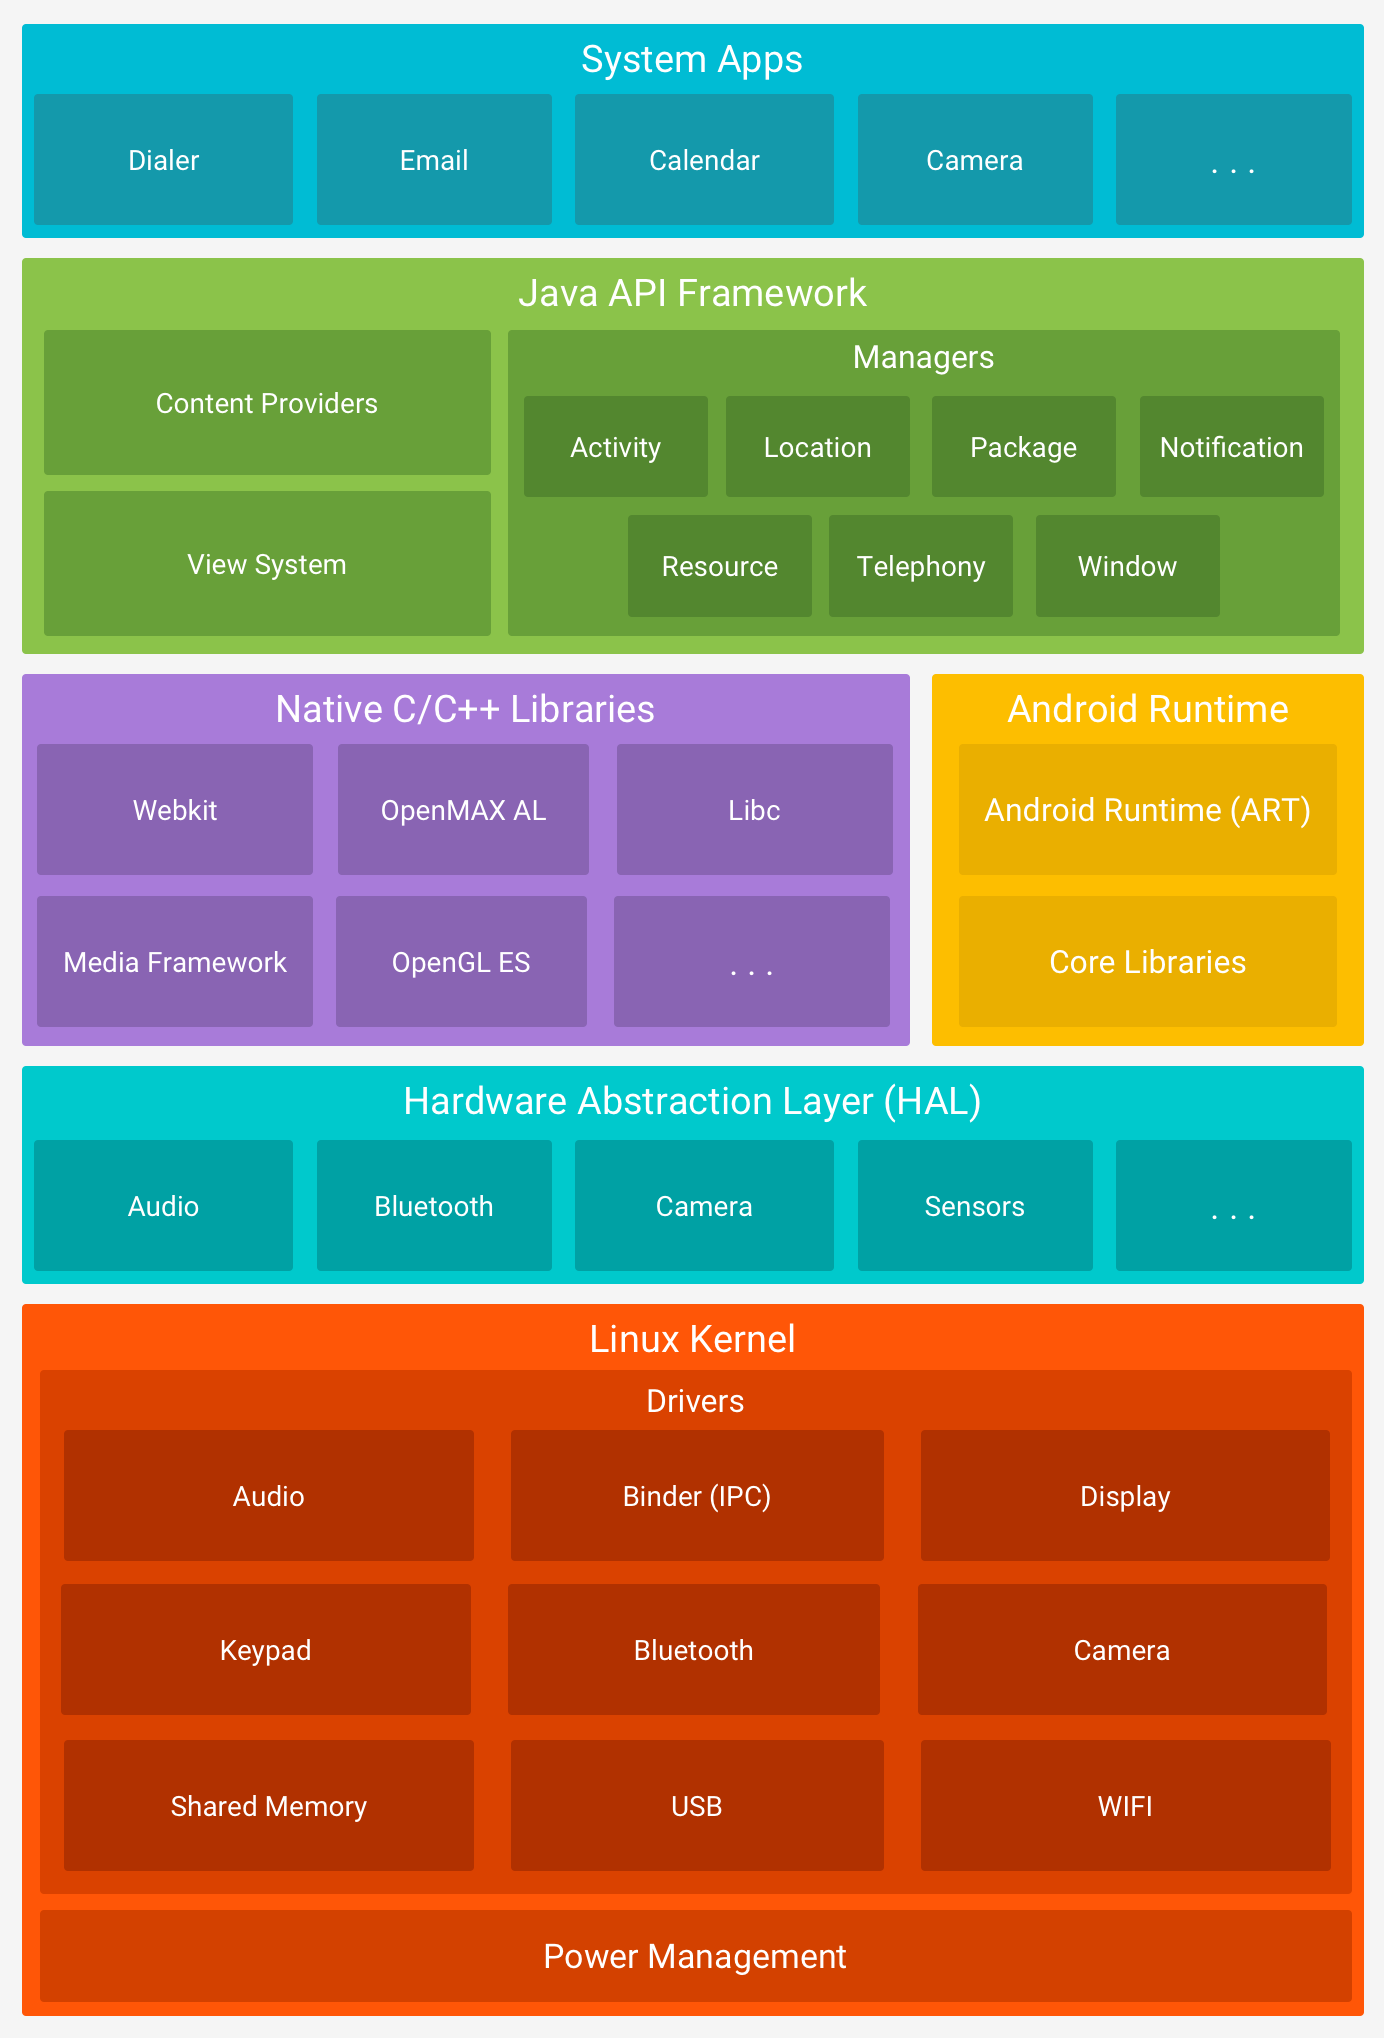
\includegraphics[width=0.7\textwidth]{Abbildungen/android-stack.png}
\caption[Android Architektur]{Die Android Architektur. (Quelle: \citet{android:architecture})}
\label{fig:android-stack}
\end{figure}\\
Die Grundlage eines Android Systems bildet dabei der Linux-Kernel, der es Android unter anderem erlaubt auf die Sicherheitsfunktionen des Kernels zuzugreifen \citep{android:architecture}. \\
Die Hardware Abstraktionschicht (HAL) stellt dem übergeordneten Java-API-Framework Standardschnittstellen zur Verfügung, über die eine Anwendung auf die Hardwarefunktionen des Gerätes zugreifen kann \citep{android:architecture}.
Übergeordnet finden sich die Laufzeitumgebung Android Runtime (ART) und nativen Bibliotheken auf. Bei letzteren handelt es sich um Biblioptheken, welche in C und C++ geschrieben sind \citep{android:architecture} und dem Entwickler unterschiedliche Funktionen zur Verfügung stellen. Die in C oder C++ geschriebenen Bibliotheken sind vor allem aus Geschwindigkeitsaspekten relevant. \\
Die Entwicklung von Android Anwendungen erfolgt dabei über das Java-API-Framework, welches dem Entwickler ein Grundgerüst sowie alle wichtigen Funktionen und Anwendungsbausteine die Für die Entwicklung relevant sind zur Verfügung stellt \citep{android:architecture}.\\
Die oberste Schicht stellen die System Anwendungen dar, bei welchen es sich um Standard-Anwendungen handelt, die Android dem Nutzer zur Verfügung stellt.

\subsection{Grundlegende Konzepte}
Alle Android Anwendungen basieren auf den selben Komponenten und Konzepten, die im folgenden einmal grundlegend betrachtet werden. Diese Komponenten sind als Klassen in Android verankert und können mittels Vererbung in Projekte eingebunden und angepasst werden 

\subsubsection{Activities}
Activities (deutsch: \glqq Aktivitäten\grqq ) stellen die Grundlage jeder Android Anwendung dar und werden durch die Klasse Activity implementiert. Dabei erzeugt jede Activity ein Fenster der Anwendung und ersetzt gleichzeitig die aus der Programmierung mit unter anderem Java bekannte main() Methode \citep{android:activities}. Anstelle einer main() Methode werden verschiedene callback Methoden aufgerufen, die einen bestimmten Zustand im Lebenszyklus einer Activity repräsentieren \citep{android:activities}. Der gesamte Lebenszyklus einer solchen Activity wird in in Abbildung \ref{fig:activity-lifecycle} dargestellt. 
\begin{figure}[h!]
\centering
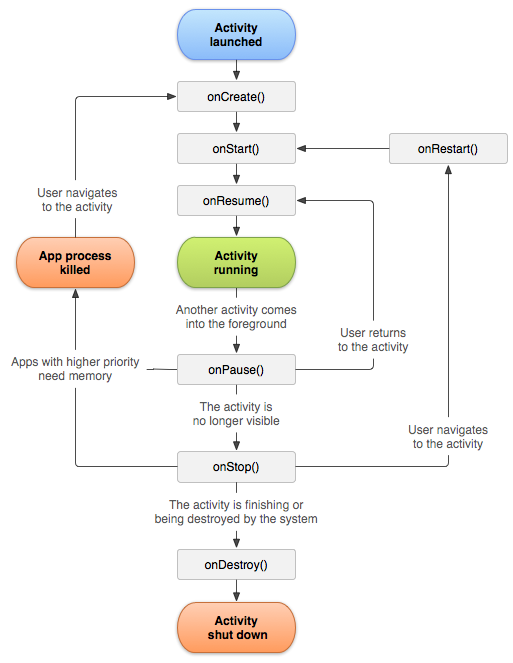
\includegraphics[width=0.7\textwidth]{Abbildungen/activity-lifecycle.png}
\caption[Lebenszyklus einer Aktivität]{Der Lebenszyklus einer Aktivität. (Quelle: \citet{android:activity-lifecycle})}
\label{fig:activity-lifecycle}
\end{figure}\\

\subsubsection{Services}
Ein Service (deutsch: \glqq Dienstleistung\grqq ) ist eine Komponente die im Hintergrund läuft und dazu konzipiert wurde langfristige Operationen auszuführen \citep{android:fundamentals}. Services können dabei unabhängig jeglicher Aktivitäten im Hintergrund laufen, auch wenn die Anwendung geschlossen wurde \citep{murphy:beginning-android}.

\subsubsection{Content Providers}
Content Providers (deutsch: \glqq Inhaltsanbieter\grqq ) stellen ein Abstraktionslevel für Daten dar, auf die aus mehreren Anwendungen zugegriffen wird\citep{murphy:beginning-android}. Mit ihrer Hilfe ist es möglich eigene Daten anderen Anwendungen zur Verfügung zustellen \citep{murphy:beginning-android}. \\
Dabei wird das Ziel verfolgt das Zusammenspiel zwischen verschiedenen Anwendungen zu verbessern, und den Datenaustausch zwischen ihnen zu verbessern.

\subsubsection{Intents}
Bei einem Intent (deutsch: \glqq Absicht\grqq ) handelt es sich um eine asynchrone Systemnachricht, die dazu genutzt werden kann bestimmte Komponenten oder bestimmte Komponentenarten zu aktivieren \citep{android:fundamentals}.

\section{OpenGL}\label{OpenGL}
OpenGl stellt die industriell meistgenutzte Programmierschnittselle (API) zur Entwicklung von 2D und 3D Anwendungen dar \citep{khronos:opengl-overview}. Mit Hilfe des Interfaces lassen sich komplexe dreidimensionale Objekte darstellen.

\subsection{Grundlagen von OpenGL}
Alle Objekte werden in OpenGL aus einem oder mehreren Polygons zusammengesetzt \citep[S. 5]{shreiner:opengl}.\\
Dabei wird jedes Poligon durch eine Menge an Eckpunkten (Vertices) definiert und jeder Eckpunkt(Vertex) stellt dabei eine Menge an Daten für einen bestimmten Punkt in einem dreidimensionalen Koordinatensystem dar \citep{vries:learn-opengl-triangle}. 

\subsection{Rendering-Pipeline} Die folgende Abbildung \ref{fig:rendering-pipeline} zeigt die Rendering-Pipeline von OpenGL. Alle Objekte und Modelle, die mit Hilfe von OpenGL dargestellt werden, durchlaufen diese Pipeline. 
\begin{figure}[h!]
\centering
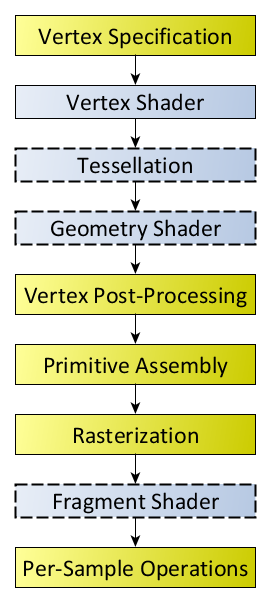
\includegraphics[width=0.3\textwidth]{Abbildungen/rendering-pipeline-opengl.png}
\caption[OpenGL Rendering Pipline]{Die Rendering-Pipeline von OpenGL. (Quelle: \citet{khronos:rendering-pipeline})}
\label{fig:rendering-pipeline}
\end{figure}\\
Die Objekte werden dabei durch eine Menge an Vertices definiert. Die zwei wichtigsten Eingriffspunkte in der Rendering-Pipeline sind der sec:vertex-shader und der sec:fragment-shader. Beide können von Programmierer implementiert werden und dienen dem Zweck verschiedene Operationen auf den einzelnen Vertices beziehungsweise den Pixeln durchzuführen. Um beide nutzen zu können müssen sie mit einem Shader Programm verknüpft werden, welches den Output von jedem Shader mit dem Input des nächsten Shaders verbindet \citep{vries:learn-opengl-triangle}.\\
Im folgenden werden einmal die einzelnen Schritte der Pipeline genauer betrachtet.\\
Bevor das Objekt dargestellt werden kann muss es zunächst definiert werden. Dieser Schritt wird als \textbf{Vertex Specification} bezeichnet. Dazu muss das Modell in viele einzelne Dreiecke unterteilt werden, welche zusammen das gesamte Objekt bilden. Diese einzelnen Flächen werden als Grundelemente (Primitives) bezeichnet \citep{khronos:rendering-pipeline} und können durch jeweils drei Eckpunkte (Vertices) beschrieben werden (siehe Abbildung \ref{fig:opengl-trangle}).
\begin{figure}[h!]
\centering
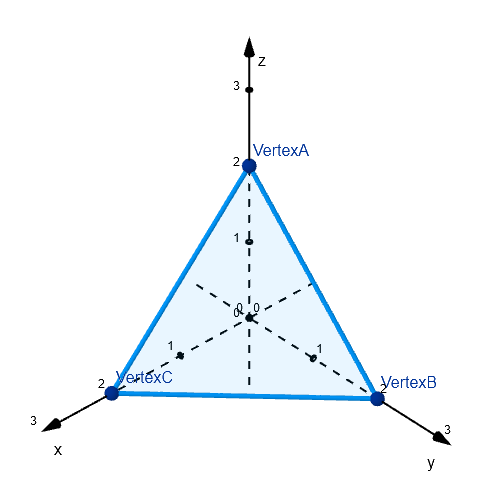
\includegraphics[width=0.3\textwidth]{Abbildungen/triangle.png}
\caption[OpenGL Triangle]{Zusammensetzung eines einzelnen Dreiecks. (Quelle: Eigene Darstellung}
\label{fig:opengl-trangle}
\end{figure}\\
\todo{Tool angeben?}
Dabei können jedem Vertex neben der Position, auch weitere Eigenschaften, welche für die Berechnungen in den nächsten Schritten der Rendering-Pipeline notwendig sind, wie Texturkoordinaten zugeordnet werden. \\
Alle Informationen werden in einer Listenstruktur gespeichert und werden im Anschluss an den \textbf{Vertex Shader} übergeben.
Dieser verarbeitet jeden einzelnen Eckpunkt, indem er bestimmte Operationen auf diesem durchführt bevor er an den nächsten Schritt der Rendering Pipeline weitergegeben wird. \citep{vries:learn-opengl-triangle}. Dabei können einzelne Attribute des Punktes transformiert werden, während andere einfach nur weitergeleitet werden.\\
Die \textbf{Tessellation} stellt einen weiteren, optionalen Schritt in der Pipeline dar. Er arbeitet mit einer Menge an Vertices, die als Patch bezeichnet wird und erzeugt aus diesen kleinere Grundelemente \citep{khronos:tessellation}. Mit Hilfe dieser Zerkleinerung können Geometrien, wie zum Beispiel Rundungen verstärkt werden.\\
Der nächste Schritt in der Rendering Pipeline ist der \textbf{Geometry Shader}, welcher ebenfalls eine optionale Station darstellt und vor allem für das Layered Rendering, bei welchem ein Grundelement in mehreren Bildern gerendert wird, genutzt werden kann \citep{khronos:geometry-shader}. 
Im Anschluss folgt das \textbf{Vertex Post-Progressing}, welches aus einer Reihe fester Funktionen besteht \citep{khronos:rendering-pipeline}, die im Kontext dieser Arbeit nicht zu brachten sind.
Der nächste Schritt ist das \textbf{Primitive Assembly} bei welchem aus der Reihe an Vertices eine geordnete Sequenz an Grundelementen geformt wird \citep{khronos:rendering-pipeline}. 
Während der \textbf{Rasterization} werden dann die Grundelemente in eine Pixeldarstellung für den entsprechenden Bildschirm umgewandelt \citep{vries:learn-opengl-triangle}.\\
Der \textbf{Fragment Shader} ordnet dann jedem Pixel eine Farbe zu, in deren Berechnung meist Werte wie Schatten, Licht und dessen Farbe einfließen \citep{vries:learn-opengl-triangle}.
Zu letzt werden dann noch eine Reihe an \textbf{Per-Sample Operations} durchgeführt, welche Tests beschreiben die testen, ob ein Pixelwert aktualisiert werden muss oder nicht \citep{khronos:rendering-pipeline}.





